% !TEX root = ../thesis.tex
% \pdfbookmark[0]{Acronyms}{Acronyms}
\chapter{Basics}
\section{Data}
There are many places to store data on a typical computer like 
a hard drive ( or any other secondary storage ), RAM, Caches 
and Registers.\\\\A hierarchy is decided on their access speed. 
If a piece of data is required more frequently, it is stored on 
a faster storage device. ( Faster implies lower latency i.e. time 
taken from being asked for data and providing it ). The figure 1 
shows this heirarchy.\\

\begin{figure}
    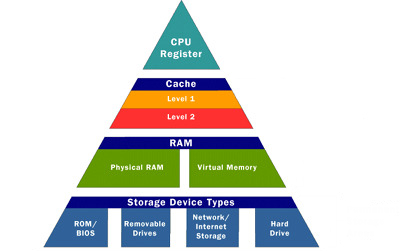
\includegraphics[width = 0.50\textwidth, center]{gfx/storageHierarchy.jpg}    
    \caption{Latency Hierarchy}
\end{figure}

\subsection*{Location}

\subsubsection*{Register}
A register is located in the CPU itself and as it is physically the
closest, it also the fastest. It is the one that is accessed while
running a program\\\\ A sample data flow can be seen in Figure 2, which shows
data tranfer from RAM to Register and then to the CPU.

\begin{figure}
    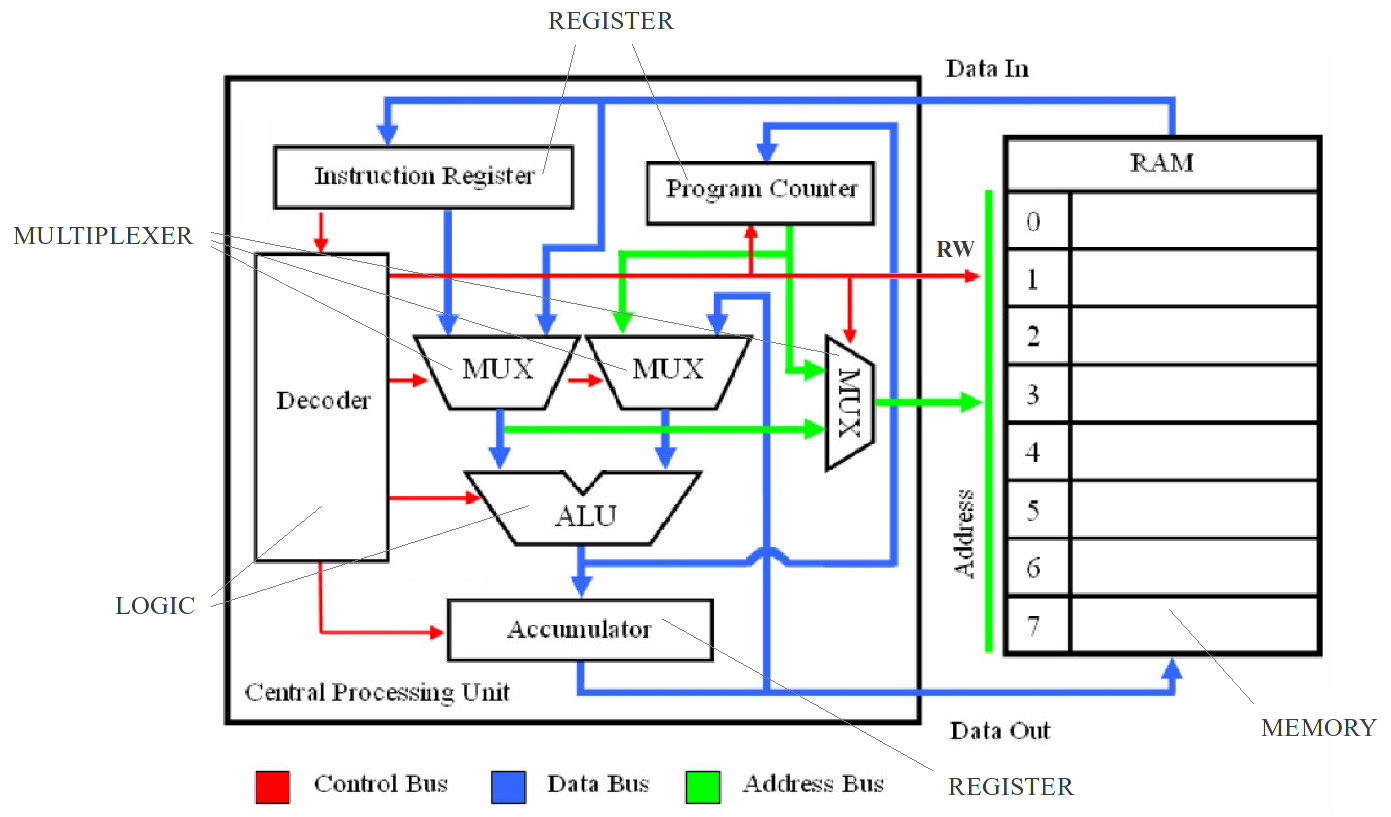
\includegraphics[width = 0.9\textwidth, center]{gfx/cpu.jpg}    
    \caption{Circuit of CPU}
\end{figure}

\subsubsection*{Cache}
A cache is small piece of memory located near the CPU and works as a
faster RAM (sort of). It caches the data which the OS thinks is required 
the most.\\\\L1 \& L2 cache is built into the proccessor (recent ones anyway) 
and is individual for every physical core whereas L3 cache is located
outside of the actual silicon but is in the chip and so is common for 
all cores.

\subsubsection*{RAM}
RAM is a volatile memory where all the memory that is deemed by the 
OS as required is stored for instant access with the CPU. The data 
tranfer happens from RAM $\rightarrow$ Cache $\rightarrow$ Register.

\subsection*{Bridges}
Bridges are small microcontrollers with built in logic which help in 
communication with external devices. There are two of there, and are 
descibed by their position on the board and also the threshold speed 
they can manage.
\subsubsection*{North Bridge}
 North bridge is a controller chip which connect high speed external 
 devices to the chipset. It was originaly outside ot the main chip 
 and an external silicon but now is mostly included in the SoC ( System on
 a chip ). The devices which can be connected to it are given in 
 Figure 3.

 \begin{figure}
    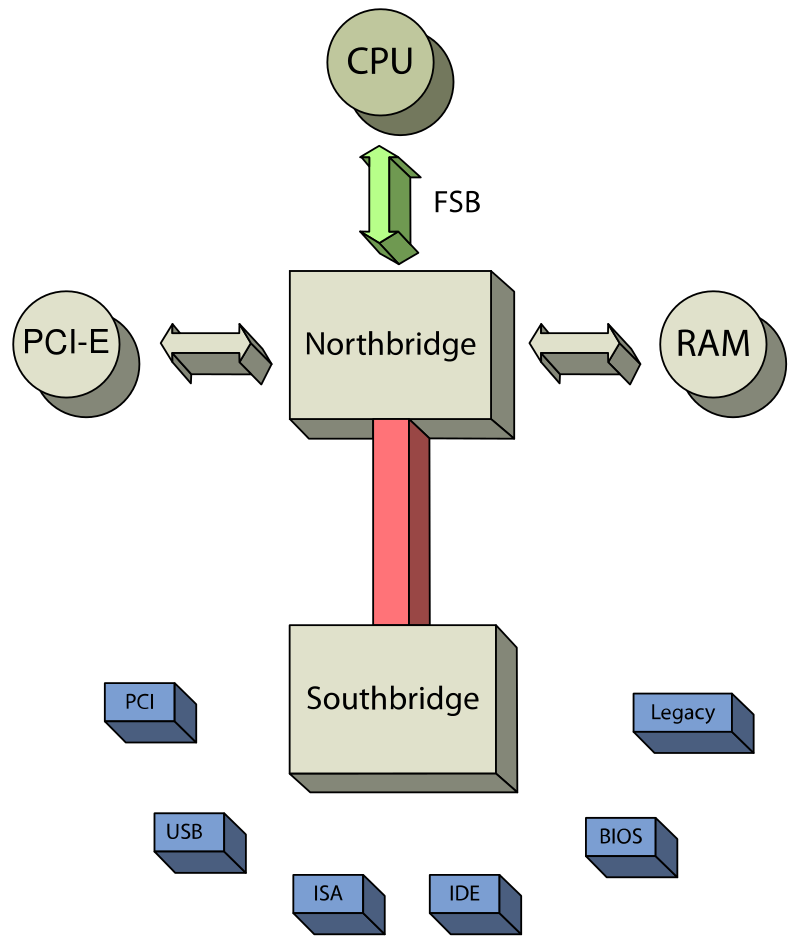
\includegraphics[width = 0.50\textwidth, center]{gfx/ChipSchem.png}    
    \caption{Use of bridges}
\end{figure}

\begin{figure}
    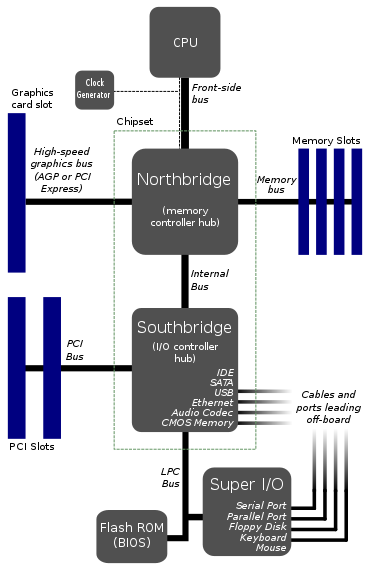
\includegraphics[width = 0.50\textwidth, center]{gfx/Motherboard.png}    
    \caption{Schematic Design of Bridges}
\end{figure}

\subsubsection*{South Bridge}
South bridge is the chipset which connects slower and legacy devices 
to the main chip. It is still seperate on Intel boards but is now 
starting to get integrated in AMD motherboards.

\subsection*{Data Flow}
So the data flow happens as follows :
\begin{center}$Solid\ State \rightarrow South\ Bridge \rightarrow RAM 
\rightarrow Register $
\end{center}
So when a computer is started, it first POSTS and then goes to 
the BIOS after which the BIOS piont the program to the Magic Number 
( For legacy MBR systems ) which has the bootloader in it (Like GRUB), 
after which the bootloader takes control of the System, then loades the 
kernel and with that the OS, which loads itself in the RAM, for fast 
access (The most recently executed programs still in the registers and 
cache) after which the OS loads a GUI ( If it has one ) or just greets 
to a TTY terminal. For the non GUI version, it gets you to a log in 
screen, whicle for GUI an application is loaded which takes care of 
logging in ( Known as a Display Manager (DM) ).

\begin{figure}
    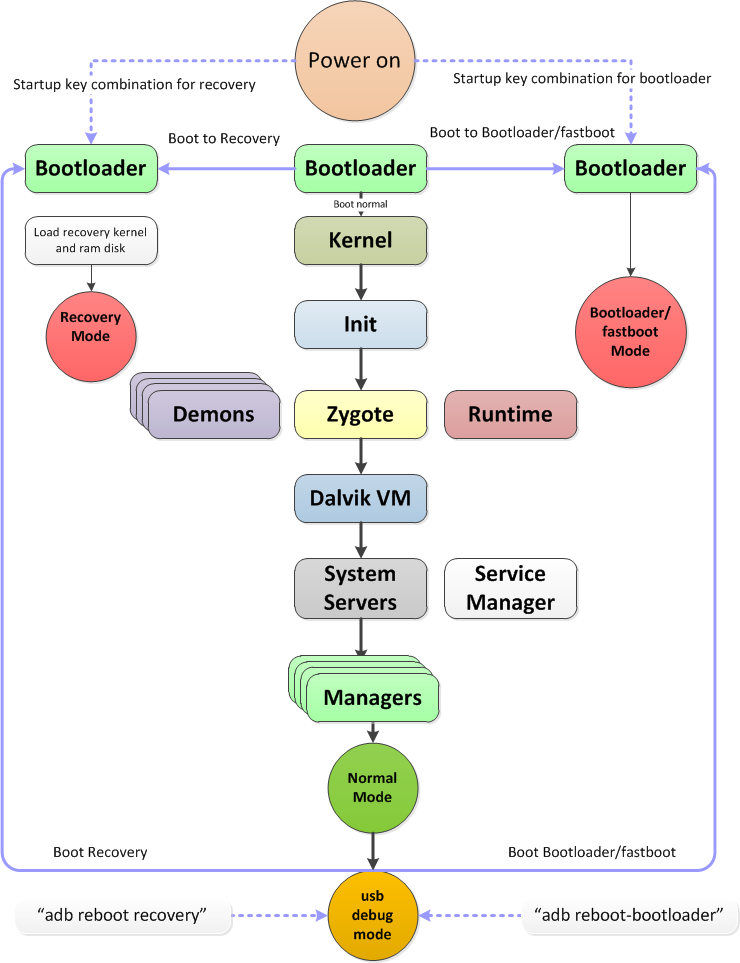
\includegraphics[width = 0.60\textwidth, center]{gfx/android-booting-process.png}    
    \caption{Android booting process}
\end{figure}
